\chapter{Objetivos}\label{cap.Objetivos}
En este capitulo se van a explicar los objetivos a conseguir y el metodo utilizado para llegar a ello.

\section{Objetivo principal}
\hspace{1 cm} El objetivo propuesto para este trabajo era conseguir que un drone navegara de forma aut\'onoma. Para ello la idea era situar el drone en un punto de inicio, despegara sobre este y una vez se hubiera estabilizado comenzara a desplazarse siguiendo un algoritmo de b\'usqueda previamente programado. La idea de este es recorrer determinado area sin la necesidad de pilotar el drone. Los movimientos de este drone dependerian de lo que detectara la c\'amara en cada momento. Esta b\'usqueda se realizar\'ia con la finalidad de encontrar una baliza sobre la cual aterrizar. En caso de no ver la baliza, el drone se moveria realizando una espiral en busqueda de esta, en el caso de encontrarla el drone se situar\'ia sobre esta y una vez centrado aterrizar\'ia. Esta baliza seria un cuadrado formado por cuatro cuadrados de colores distintos. 

\begin{figure}[H]
	\centering
		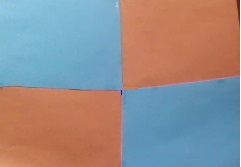
\includegraphics{imgs/baliza.jpg}
	\label{fig:Baliza elegida sobre la que aterrizar. }
\end{figure}

\hspace{1 cm} Para conseguir este objetivo, hay que tener en cuenta varias partes importantes, de las cuales a partir de una pasamos a la otra para al final llegar a lo que permitir\'a el correcto funcionamiento del algoritmo: que los movimientos de este dependan de lo que ve la c\'amara.

\begin{itemize}
	\item \textbf{Creaci\'on de un filtro de color:} Gracias a los colores podemos detectar los cuadrados de la baliza, por lo que realizando este filtro obtendremos estos objetos y los que sean del mismo color, eliminando as\'i informaci\'on no necesaria de la imagen.
	
	\item \textbf{Detecci\'on de objetos: } Tras el filtro de color y eliminada informaci\'on no necesaria, podemos obtener distintos objetos en la imagen, viendo si cumplen caracter\'isticas como tener un determinado area, para as\'i saber si son los objetos que se desean o no y trabajar con ellos o descartarlos. 
	
	\item \textbf{Movimiento del drone: } Una vez obtenemos informaci\'on de la imagen y la hemos procesado, en funci\'on de esto se pretender\'a que el desplazamiento del drone sea uno u otro, trabajando asi de forma fluida y sin movimientos bruscos que puedan desestabilizarlo.   

\end{itemize}


\section{Metodolog\'ia}
\hspace{1 cm} Para poder conseguir todo esto, era necesario saber las plataformas con las que ser\'ia posible, donde tiene gran importancia el software JdeRobot, pues gracias a su desarrollo que permite la comunicaci\'on con el dron, y de estas forma obtener los datos de sus sensores, principalmente de la camara. Para este apartado fue primordial el aprendizaje de sus distintas herramientas, hubo que hacer pruebas con estas y ver su funcionamiento tanto en entornos simulados como en reales.

\hspace{1 cm}Una vez se realizaron las primeras pruebas con robots, se propuso un desarrollo en espiral. Para este desarrollo se proponian semanalmente reuniones con el tutor, en las cuales se proponian unos objetivos a seguir en funci\'on de lo que se hab\'ia conseguido hasta el momento. Una vez propuestas estas tareas se evaluavan los distintos riesgos que se pod\'ian tomar en funci\'on de trabajar de una forma u otra, y los avances a los que se pod\'ia llegar por cada camino. Una vez hecho esto se comenzaban a desarrollar los algoritmos para conseguir estos objetivos en funci\'on de la forma elegida. Una vez se realizaban estos y se probaban (en simulaci\'on o con el robot real, dependiendo del objetivo), se propon\'ia otra reuni\'on para determinar si los avances eran los deseados o no, y en funci\'on de esto planear unos objetivos u otros.  

\begin{figure}[H]
	\centering
		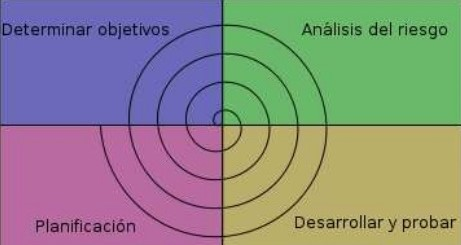
\includegraphics{imgs/metodologia-espiral.jpg}
	\label{fig:Desarrollo en espiral}
\end{figure}

\hspace{1 cm} Los avances que se iban realizando semana a semana, se subian mediante videos o imagenes a un mediawiki en JdeRobot, quedando reflejados todos los procesos. Tambi\'en se ha utilizado GitHub para subir el c\'odigo desarrollado.  

\section{Plan de trabajo}
\hspace{1 cm} El primer punto fue comprender las distintas herramientas de JdeRobot y trabajar con ellas. Creando programas simples y viendo que funcionaban, as\'i como trabajar con distintos robots reales para tener una toma de contacto con ellos y no basarse solo en un trabajo sobre simulador. 

\hspace{1 cm} En segundo lugar hubo que comprender la importancia que tendria la biblioteca OpenCV en este proyecto y ver sus multiples opciones, todo lo que permitia trabajar con imagenes y los cambios que podiamos hacer sobre estas para obtener datos deseados a partir de los cuales mandar informaci\'on. 

\hspace{1 cm} Por ultimo quedaba unir estas dos tecnolog\'ias y conseguir un buen algoritmo que nos permitiera enviar informaci\'on a tiempo real a un drone y que este la ejecutara de forma correcta y fluida.  




